% Template for a Computer Science Tripos Part II project dissertation
\documentclass[12pt,a4paper,twoside,openright]{report}
\usepackage[pdfborder={0 0 0}]{hyperref}    % turns references into hyperlinks
\usepackage[margin=25mm]{geometry}  % adjusts page layout
\usepackage{graphicx}  % allows inclusion of PDF, PNG and JPG images
\usepackage{verbatim}
\usepackage{pdfpages} % allows inclusion of non tex project proposal
\usepackage{docmute}   % only needed to allow inclusion of proposal.tex
\usepackage{tikz}
\usetikzlibrary{shapes,arrows,positioning,chains}

\raggedbottom                           % try to avoid widows and orphans
\sloppy
\clubpenalty1000%
\widowpenalty1000%

\renewcommand{\baselinestretch}{1.1}    % adjust line spacing to make
                                        % more readable
\begin{document}

\bibliographystyle{plain}


%%%%%%%%%%%%%%%%%%%%%%%%%%%%%%%%%%%%%%%%%%%%%%%%%%%%%%%%%%%%%%%%%%%%%%%%
% Title


\pagestyle{empty}

\rightline{\LARGE \textbf{Oliver Black}}

\addcontentsline{toc}{chapter}{Cover Sheet}

\vspace*{60mm}
\begin{center}
\Huge
\textbf{Software IPv6 Router in Rust} \\[5mm]
Computer Science Tripos -- Part II \\[5mm]
Selwyn College \\[5mm]
\today  % today's date
\end{center}

\newpage
\addcontentsline{toc}{chapter}{Declaration of Originality}
\section*{Declaration of Originality}

I, Oliver Black of Selwyn College, being a candidate for Part II of 
the Computer Science Tripos, hereby declare
that this dissertation and the work described in it are my own work,
unaided except as may be specified below, and that the dissertation
does not contain material that has already been used to any substantial
extent for a comparable purpose.

\bigskip
\leftline{Signed Oliver Black}

\medskip
\leftline{Date \today}

%%%%%%%%%%%%%%%%%%%%%%%%%%%%%%%%%%%%%%%%%%%%%%%%%%%%%%%%%%%%%%%%%%%%%%%%%%%%%%
% Proforma, table of contents and list of figures

\pagestyle{plain}

\chapter*{Proforma}
\addcontentsline{toc}{chapter}{Proforma}

{\large
\begin{tabular}{ll}
Name:               & \bf Oliver Black                      \\
College:            & \bf Selwyn College                     \\
Project Title:      & \bf Software IPv6 Router in Rust \\
Examination:        & \bf Computer Science Tripos -- Part II, July 2001  \\
Word Count:         & \bf "FIX ME\& footnote" \footnotemark[1]
                       \\
Project Originator: & Oliver Black \& Dr Richard Watts      \\
Supervisor:         & Andrew Moore                   \\ 
\end{tabular}
}
\footnotetext[1]{This word count was computed
by \texttt{detex diss.tex | tr -cd '0-9A-Za-z $\tt\backslash$n' | wc -w}
}
\stepcounter{footnote}


\section*{Original Aims of the Project}

The IPv6 standard contains a large number of complex requirements, complicating understanding. I aim to design and implement a simple IPv6 router using Rust\cite{rust} that behaves as specified in the IPv6 RFCs\cite{ipv6_rfc}. This router should implement the minimum functionality required by the relevant standards, yet still be functional, minimal, \& stable.  Rust is a new programming language that aims to be as fast as C while maintaining memory safety, I wanted to understand how practical it was to develop in.

\section*{Work Completed}

Despite having initial difficulties setting up my test environment using Mininet\cite{mininet}, due to its lack of support for IPv6, I successfully implemented a functioning IPv6 router in rust that met almost all of my core requirements. Both the router itself, and the test bench, are available for public use.  TODO mention speedup/code coverage/size/RFC coverage/throughput AND fill rest in when main body done. mention how ambitious original claims were

\section*{Special Difficulties}

None. TODO fill in

\tableofcontents
\addcontentsline{toc}{chapter}{Table of Contents}
\listoffigures
\addcontentsline{toc}{chapter}{List of Figures}

\newpage
\section*{Acknowledgements}

Many thanks to:
\begin{itemize}
\item My supervisor Andrew Moore for his helpful advice.
\item My Director of Studies Dr Richard Watts for his guidance.
\item Friends \& family for proofreading.
\end{itemize}

%%%%%%%%%%%%%%%%%%%%%%%%%%%%%%%%%%%%%%%%%%%%%%%%%%%%%%%%%%%%%%%%%%%%%%%
% now for the chapters

\pagestyle{headings}

\chapter{Introduction}
\label{chap::introduction}
Slowly but surely the internet is making progress towards IPv6, but how do pages of Requests for Comments (RFCs) translate into real world network components? The aim of this project was to develop an IPv6 Router in Rust that explores the functionality of IPv6, and how different parts of the various standards fit together. The project has been a success, I have produced a functioning router and accompanying test suite.

\bigskip

Due to the popularity of the Internet, there are now not enough IPv4 addresses to go around. IPv6 is the incoming internet addressing standard that solves numerous issues with IPv4.  Primarily it increases the number of addresses, however it also fixes many flaws in the IPv4 design, and standardises common non-standard practices. For example, the Time To Live in IPv4 was defined partly in terms of seconds left to live\cite{ipv4_rfc}, but in practice was just decremented by 1 on every hop between nodes. In IPv6 the field is accurately renamed to Hop Limit, and is now defined in terms of hops between nodes (as opposed to seconds). Many subtle decisions like this have gone into the IPv6 standard, with an aim to making an internet that works well, rather than one that just works.

\bigskip

Rust\cite{rust} is an up and coming modern low level programming language. It aims to match the performance of C/C++ without sacrificing memory safety, and avoiding garbage collection. It does this through zero-cost high level abstractions such as \textit{ownership} and \textit{lifetimes}. For example, if you pass something to a function, that function then owns that and everything it owns, with it being inaccessible after the function returns. It is possible for functions to borrow values instead, using ``\texttt{\&}'', similar to passing by reference.  I chose Rust for my project as it can be easier to debug than C or C++, but mainly because I was interesting in learning Rust.

\bigskip

Mininet\cite{mininet} is an open source virtual network simulator that was developed at Stanford and until 2016 was used in the Part 1B Computer Networking course, it is written in Python.  It creates lightweight virtual networks by making use of Linux's \textit{networked namespaces}, allowing processes to share a kernel, yet be behind different network interfaces. This made it the ideal candidate to build my router and test suite on top of. A simple IPv4 router\cite{simple_router} already exists, and can be ran on top of Mininet, it explores how IPv4 works quite effectively.  Seeing this was one of the key inspirations for my project.

\bigskip

Routers are the backbone of the internet, at the most simple level many of them have a \textit{control plane} that deals with addressing, and a \textit{forwarding plane} that deals with actually sending packets. There are many open source routers out there, but almost all of them have lots of IPv4 code. This makes it difficult to isolate and understand how the IPv6 part actually works.  Starting from scratch allows you to avoid having to deal with IPv4 at all.  

\bigskip

Using the IPv6 standard as a framework, combined with some knowledge about the internals of routers, it is possible to develop and IPv6 router that is stable, small, simple, \& fast.  Such a router could continue to be developed until it could be deployed on actual hardware, but the implementation and testing required meant this was not an objective of this project.  Instead, the aim is to develop a router that implements a sub-set of the IPv6 standard, hopefully including everything an IPv6 router is required by the standards to implement.  In the remainder of this dissertation I will discuss the preparation, implementation, and evaluation of this project.

\chapter{Preparation}

Before starting the implementation lots of research and design needed to be done. Lots of research was done into IPv6 RFCs and which aspects were required to be implemented, and which were not. The router software was then designed to provide a framework within which these aspects could be implemented.  Additionally a test plan needed to be made, to enable effective evaluation of the finished product.

\section{Starting Point}
This project was in areas I was interested in and had some experience in. Those areas were all, however, approached from new angles:
\begin{itemize}
\item \textbf{Low-level Systems Programming:} As well as the Part 1B C course I had done several internships that involved a substantial amount of low-level programming in C. However I had never written any project in Rust before.
\item \textbf{Network Programming:} I had completed the Part 1B Computer Networking course, so had some theoretical understanding.  I had also worked on side assignment of a large networking project during an internship.  However I had never worked on a networking project by myself from the ground up before.
\item \textbf{Testing:} I had obviously written tests for my own code before, and had been exposed to large testing frameworks during internships.  However I had never devised my own formal test plan and developed my own test bench before.
\end{itemize}

\section{Research}
An analogous project for IPv4 called Simple Router already exists\cite{simple_router} (it used to be a recommended extension task for the Part 1B Computer Networking course).  It is implemented in C, but it ran on top of Mininet.  The implementation didn't help at all (due to being in C and for IPv4), but it running on Mininet demonstrates that running a router on Mininet is feasible.  Additionally the Mininet python code that ran the Simple Router's executable helped me in designing my test bench.

\bigskip

Most of my research time however was spent reading RFCs related to IPv6.  The main RFC\cite{ipv6_rfc} specifies everything you need to know about IPv6 packets. This describes the contents of the main IPv6 header, \hyperref[fig::ipv6_header]{Figure }\ref{fig::ipv6_header}, including how the fields (e.g. \textit{Hop Limit}) are modified for packets in transit. Additionally this includes the extension headers that need to be implemented by a router, when the packet in question is not addressed to the router this turns out to be none. 

\begin{figure}
\begin{verbatim}
+-+-+-+-+-+-+-+-+-+-+-+-+-+-+-+-+-+-+-+-+-+-+-+-+-+-+-+-+-+-+-+-+
|Version| Traffic Class |           Flow Label                  |
+-+-+-+-+-+-+-+-+-+-+-+-+-+-+-+-+-+-+-+-+-+-+-+-+-+-+-+-+-+-+-+-+
|         Payload Length        |  Next Header  |   Hop Limit   |
+-+-+-+-+-+-+-+-+-+-+-+-+-+-+-+-+-+-+-+-+-+-+-+-+-+-+-+-+-+-+-+-+
|                                                               |
+                                                               +
|                                                               |
+                         Source Address                        +
|                                                               |
+                                                               +
|                                                               |
+-+-+-+-+-+-+-+-+-+-+-+-+-+-+-+-+-+-+-+-+-+-+-+-+-+-+-+-+-+-+-+-+
|                                                               |
+                                                               +
|                                                               |
+                      Destination Address                      +
|                                                               |
+                                                               +
|                                                               |
+-+-+-+-+-+-+-+-+-+-+-+-+-+-+-+-+-+-+-+-+-+-+-+-+-+-+-+-+-+-+-+-+
\end{verbatim}
\caption{IPv6 Header Format\cite{ipv6_rfc}}
\label{fig::ipv6_header}
\end{figure}

\bigskip

Another important RFC was the Internet Control Messaging Protocol RFC\cite{icmpv6_rfc}.  This protocol accompanies IPv6 proper, and must be implemented by all IPv6 routers.  It allows, among other things, errors about dropped packets to be sent back to the source, and \textit{Echo Request/Reply} (ping) messages to be sent.  Alongside this it was important to gain an understanding of how IPv6 related to the link layer below and the transport layer above.

\bigskip

The IPv6 Addressing RFC\cite{ipv6_rfc_adr} contains all you could want to know about the various kinds of IPv6 addresses. However, it is mainly just a list of address ranges and whether they have any special behaviour, it doesn't affect the design of a router much.  I also consulted a few more RFCs related to features that didn't \textit{need} to be implemented by an IPv6 router, more details on those can be found under \hyperref[appendix::requirements]{Appendix A}.

\bigskip

Finally I spent some time researching rust, as it was a new language to me, and I didn't want to make mistakes early on in my implementation that would make things much harder later on.  I discovered a library called pnet\cite{pnet_rust} which implemented low level networking functions and packet abstractions, exactly what I would need.

\section{Analysis}

After finishing my research I needed to do some \textit{requirements analysis} to workout what exactly my router needed to implement, and in what order I should go about implementing them.  I divided up the requirements as recommended into \textit{core} and \textit{extension}, where core contained everything an IPv6 router \textit{needed} to do (according to the RFCs), and extension things I thought I would like it to do as well.  Core was further divided up into \textit{basic} and \textit{advanced}, with basic being everything the router required to provide some form of basic testable functionality, and extension being everything else that was \textit{needed}.

\bigskip

There are three main areas of requirements:
\begin{itemize}
\item Addressing
\item Packet inspection \& forwarding
\item Error reporting \& ICMPv6\cite{icmpv6_rfc}
\end{itemize}

\bigskip

The requirements for addressing can be divided into two parts, the address discovery mechanism (static, SLAAC\cite{slaac_rfc} or DHCPv6\cite{dhcpv6_rfc}) and different address types (Unicast, Anycast, Multicast).  

Although DHCPv6 and SLAAC are both practical and interesting, they aren't \textit{needed} for an RFC router - static addressing is sufficient - so they were put as extension requirements.  Static addressing means the relationship between IPv6 addresses and link layer interfaces is defined when the router starts based on a fixed configuration. In order to get the router forwarding packets as quickly as possible an additional requirement of \textit{flooding} addressing was added.  This is not defined in the RFC for IPv6, as it means the router functions instead as a link layer switch, sending all incoming packets out on all interfaces. Static addressing was \textit{needed} by the RFCs and I decided flooding alone wouldn't really constitute basic testable functionality (of a router). So static addressing is a basic core requirement, with DHCPv6 and SLAAC being extension requirements.

Address types in IPv6 are well defined by the addressing RFC\cite{ipv6_rfc_adr}, hand a router \textit{needs} to deal with all of them.  However, in order to test basic functionality only Unicast really needs to be implemented, as Anycast and Multicast are just mappings from a 'Unicast' address to many Unicast addresses. So Unicast is a basic core requirement, with Anycast and Multicast being advanced core requirements. IPv6 also includes scope for local only addresses, as well as a variety of other specific types, these could also have been extension requirements.

\bigskip

Every packet the router receives needs to be sent to the right destination, and any packet for which the destination is unknown should be sent to the default route. This falls under static addressing as my requirements don't differentiate between the control and data plane - see \hyperref[sec::design]{Design}.  However the payload length must be checked to see if it matches the actual length of the payload - and the packet discarded if not.  Additionally the hop limit must be checked, if it is 1 or 0 the packet should be discarded, otherwise it should be decreased by 1.  Both of these are basic core requirements, they are \textit{needed} and without them it is hard to test basic functionality. Without hop-limit decrements the router leaves packets unaffected, so it is hard to tell if they went through the router at all.

IPv6 also has many extension headers, but they \textit{need} to be ignored by intermediate nodes (for example, fragmentation can only be done by the source and destination nodes), except for the \textit{hop-by-hop options header} which can be ignored by intermediate nodes. Apart from ICMPv6 packets my router does not deal with packets that are encapsulated by IPv6 packets (including transport layer protocols).  This means that it does not need to process any headers at all, except for ICMPv6 packets.

\bigskip

ICMPv6 works alongside IPv6 to send informational and error messages between nodes.  These messages include destination, packet size, hop limit, \& header error messages, and echo request \& reply informational messages. One slightly odd requirement relates back to hop-limit in the IPv6 header, if an arriving packet has a hop limit of 1, it should be discarded, unless the destination node is the router.  This only occurs for ICMPv6 messages. 

ICMPv6 is /textit{needed} for any IPv6 router.  However, in order to test the basic functionality of my router it was not required. This is because error reporting functions can be, in part, replaced by log output from the router itself. As such, ICMPv6 is an advanced core requirement.

\bigskip

Additionally I thought about what my project did not need to do. I have already discussed briefly in my \hyperref[chap::introduction]{Introduction} that I did not want to require my router be able to be ran on actual hardware, as this would add needless complexity when my aim is to explore and illuminate the IPv6 requirements. 

I did not want to bother with any experimental/unused features, as they don't much help understand the IPv6 requirements. For example the flow label in the IPv6 header can in theory be used to prioritise real time packets, and several other uses have been suggested, however it can just be ignored by the standard, and I believe that is what many routers do.  The same can be applied to many IPv6 extension headers, I planned to evaluate all my extension requirements to see if they met this criterion after finishing my core requirements.

I didn't want to get involved with cross-layer optimisations, as these would also not help to understand the IPv6 requirements.  Secondly, this would not be particularly useful, as the nature of means my router has few bottlenecks, but it is often in bottlenecks that such cross-layer optimisations are used.

Mininet does allow for artificially reducing the MTU of links, and through the help of helper applications artificially dropping packets and increasing latency.  However, my aim was not to produce a high performance router, so any requirement based on performance was also not what I was looking for.

\bigskip

To summarise, here are the requirements for my router, categorised by type, starting with my basic core requirements:
\begin{itemize}
\item Send packets to the correct hardware interface in accordance with the static routing rules provided
\item Deal with IPv6 headers in accordance with the standard (Hop limit, etc)
\end{itemize}
My advanced core requirements:
\begin{itemize}
\item ICMPv6
\item Multicast
\item Anycast
\end{itemize}
My extension requirements:
\begin{itemize}
\item IPv6 extension headers
\item DHCPv6
\item SLAAC
\end{itemize}
My non-goals, things that would needlessly complicate the project:
\begin{itemize}
\item To be stable, complete, fast, \& compatible enough to be easily run on real hardware in a real world environment.
\item Implementing experimental or unused features - specifically those potentially covered by my extension requirements.
\item Higher layer packet inspection
\item Performance based goals (throughput, etc)
\end{itemize}
For a formal list of the requirements I came up with (along with identifiers and associated tests) see \hyperref[appendix::requirements]{Appendix A}.

\section{Design}
\label{sec::design}

Having completed my analysis and produced a structured list of requirements the next step was to come up with a design of router that would enable me to implement these requirements.  There were two main ideas in the design of the router itself (the design of the test bench is discussed in the next section). 

\bigskip

The first was the separation of the control and forwarding plane, which by itself is nothing special, but the design in software was slight more complex.  As always, the control plane deals with the addressing (along with other aspects and the forwarding plane with link layer interfaces and individual packets.  The two communicate through forwarding tables (in the case of non static addressing communication in the other direction is also required). The forwarding plane in my case is made up of a pair of threads for each interface, one receiving and one transmitting. All of the receiving threads have read access to two objects, one is the routing table produced by the control plane, the other is a map of hardware addresses to channels.  The channel each hardware address is linked to leads to the transmitting thread for the interface of that hardware address (See \hyperref[fig::router_design]{Figure }\ref{fig::router_design}). Read \hyperref[chap::implementation]{Implementation} for specifics.

\begin{figure}
\centering
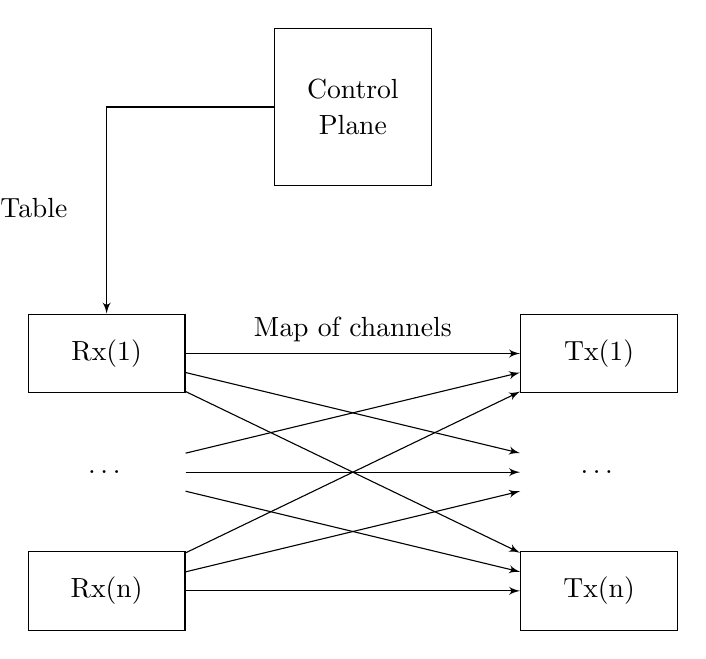
\begin{tikzpicture}
\tikzstyle{block} = [rectangle, draw, 
    text width=5em, text centered, minimum height=2cm,node distance = 2cm]
\tikzstyle{middle} = [text width=5em, text centered, minimum height=1cm,node distance = 2cm]
\tikzstyle{little} = [rectangle, draw, middle]
\tikzstyle{line} = [draw, -latex']

\node [block] (control) {Control Plane};
\node [below=of control, yshift=-10mm] (center) {};
\node [little, left=of center] (recv1) {Rx(1)};
\node [little, below=of recv1] (recv2) {Rx(n)};
\node [little, right=of center] (trans1) {Tx(1)};
\node [little, below=of trans1] (trans2) {Tx(n)};

\path (recv1) -- node [middle] (midl){\ldots} (recv2);

\path (trans1) -- node [middle] (midr){\ldots} (trans2);

\path [line] (control) -|
node [near end, transform canvas={xshift=-16mm}] {Routing Table}
(recv1);

\path  [line] (recv1) -- node [transform canvas={yshift=+3mm}] {Map of channels} (trans1);
\path  [line] (recv1) -- (trans2);
\path  [line] (recv1) -- (midr);

\path  [line] (midl) -- (trans1);
\path  [line] (midl) -- (trans2);
\path  [line] (midl) -- (midr);

\path  [line] (recv2) -- (trans1);
\path  [line] (recv2) -- (trans2);
\path  [line] (recv2) -- (midr);

\end{tikzpicture}
\caption{Router Design}
\label{fig::router_design}
\end{figure}

\bigskip

The second was designing the layer separation inherent in the TCP/IP stack into the router.  This was achieved by having a different function handle each layer, and only passing necessary information between the functions.  There are three layers, Ethernet, IPv6, and ICMPv6 in the router, so there are three functions, with only the packets themselves and the relevant addresses being passed between the functions. The Ethernet function sends the IPv6 packet to the IPv6 function, which returns the new IPv6 packet, and the hardware address to send it to.  The IPv6 function sends the ICMPv6 packet along with the source and destination address to the ICMPv6 function, which returns the new ICMPv6 packet along with the new source and destination addresses (See \hyperref[fig::layer_separation]{Figure }\ref{fig::layer_separation}).

\begin{figure}
\centering
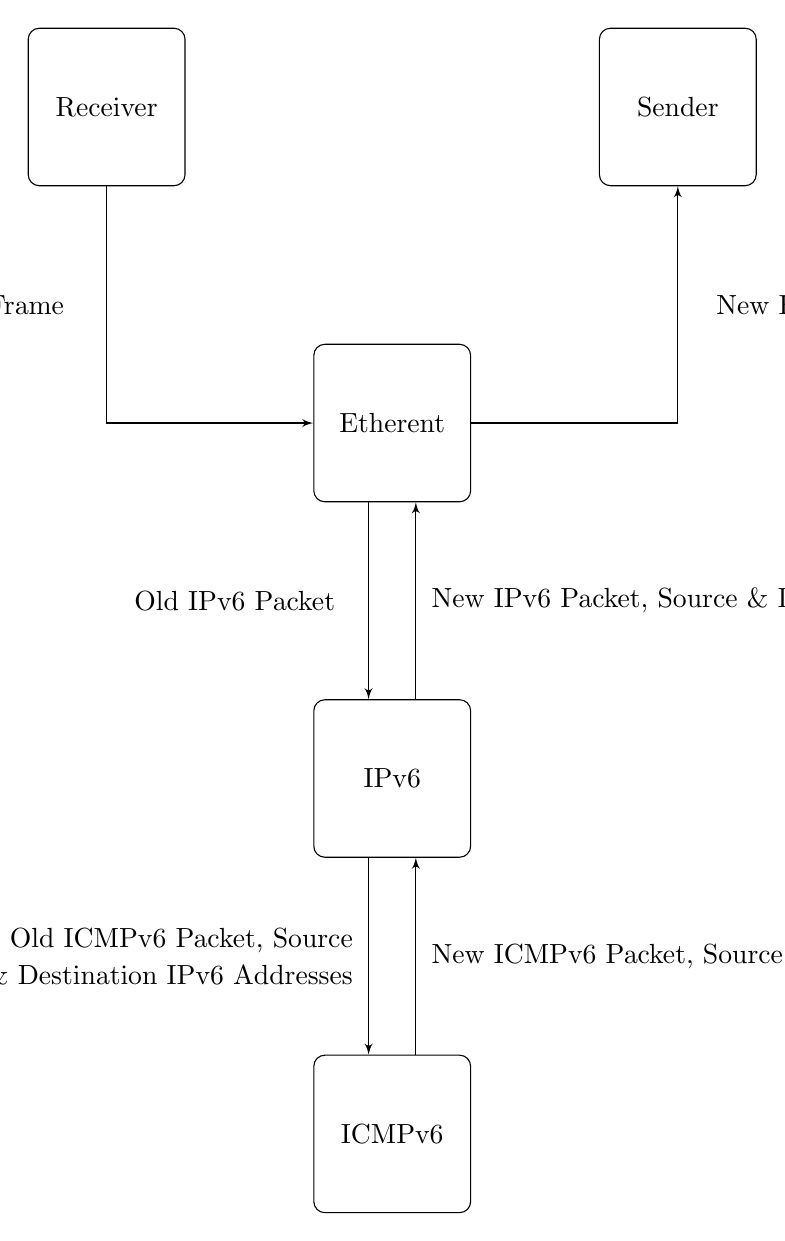
\begin{tikzpicture}

\tikzstyle{block} = [rectangle, draw, 
    text width=5em, text centered, rounded corners, minimum height=2cm,node distance = 2.5cm]
\tikzstyle{invisible} = [rectangle,minimum height=1cm]
\tikzstyle{line} = [draw, -latex']

\node [invisible] (anchor) {};
\node [block, left=of anchor] (receiver) {Receiver};
\node [block, right=of anchor] (sender) {Sender};
\node [block, below=of anchor] (ethernet) {Etherent};
\node [block, below=of ethernet] (ipv6) {IPv6};
\node [block, below=of ipv6] (icmpv6) {ICMPv6};

\path [line] (receiver) |- 
node [near start, transform canvas={xshift=-21mm}] {Old Ethernet Frame} 
(ethernet);
\path [line] (ethernet) -| 
node [near end, transform canvas={xshift=+21mm}] {New Ethernet Frame} 
(sender);
\path [line] (ethernet) edge [transform canvas={xshift=-3mm}] 
node [transform canvas={xshift=-17mm}] {Old IPv6 Packet}
(ipv6);
\path [line] (ipv6) edge [transform canvas={xshift=+3mm}] 
node [transform canvas={xshift=+42mm}, text width=8cm, align=left] {New IPv6 Packet, Source \& Destination MACs}
(ethernet);
\path [line] (ipv6) edge [transform canvas={xshift=-3mm}] 
node [transform canvas={xshift=-42mm}, text width=8cm, align=right] {Old ICMPv6 Packet, Source \& Destination IPv6 Addresses}
(icmpv6);
\path [line] (icmpv6) edge [transform canvas={xshift=+3mm}] 
node [transform canvas={xshift=+42mm}, text width=8cm, align=left] {New ICMPv6 Packet, Source \& Destination MACs}
(ipv6);
\end{tikzpicture}
\caption{Layer Separation}
\label{fig::layer_separation}
\end{figure}

\bigskip

Both of these design choices made the implementation much easier, separating the code into functionally separate sections, reducing the risk of introducing bugs, and most importantly providing a structured framework within which to code.

\section{Test Plan}

With requirements and a design of the router completed, I needed to come up with a plan of how I was going to verify that my router was functioning as expected.  This was divided into two parts, the design of the test bench, and secondly the list of tests to be run on it.

\bigskip

I planned to make up my test bench from Mininet and a couple of helper applications (either written in Python or Rust).  Some helper applications would be capable of sending packets with specific properties, and outputting any packets they received. Other helper applications would do more complicated end to end testing, such as running a web server and requesting web pages.  Unfortunately I found Mininet's IPv6 support was far less complete than I had believed in my \hyperref[project_proposal]{Project Proposal}.  I either had to write my own network emulation environment from scratch, or develop some kind of modification or wrapper for Mininet.  I chose to focus on a wrapper that would intercept the functions I needed to use, and change the necessary things to get Mininet working, details of this wrapper can be found in \hyperref[chap::implementation]{Implementation}.

\bigskip

When formalising the results of my analysis into a list of tests there were two key steps. The first, a one, was numbering everything so I wouldn't get lost or forget any requirements.  Secondly I had to think of the test themselves, this normally included a test for the given functionality when it should happen, a test for it not happening when it shouldn't happen, and any edge case tests I could thing of.  For example, hop limit decrement, when a packet passes through the router its hop limit should be decreased by 1 and the packet sent on its way; when the packet has a hop limit of 1 or 0 on arrival it should be dropped and not sent on its way, and if, the packet has a hop limit of 1 and is addressed to the router it should not be dropped, it should instead be handed up a layer. 

\bigskip

To avoid all the tests being dependent on an almost complete implementation of the router. If we return to the example hop limit given above the router should send an ICMPv6 \textit{Time Exceeded} message when a packet is dropped.  However, this would mean any test for hop limit depends on a correct implementation of ICMPv6, as well as the correct implementation of Hop Limit.  As a result every test can only rely on functionality already implemented.  My numbering system happened to match my planned order of implementation, so just reading off all the previous tests lets you know which features that test potentially relies on.  Back to the hop limit example, this means that success of the hop limit test was judged by the packet not continuing and log messages being outputted by the router process. When it came to test Time Exceeded though it could rely on the already implemented hop limit, so the planned test involved sending a packet with hop limit 0 and testing for a Time Exceeded response.

\section{Professional Practice}
This is a brief section on issues related to professional 

\chapter{Implementation}
\label{chap::implementation}

Implementing my router was an exciting iterative process, with every

\section{Router}

explain design into practice

static addressing

Code for threads
Code for separation
Code for multithreaded routing table

\section{Test Bench}

Mininet

Mention flooding success then test plan stuff - maybe in router?


Maybe some stuff from evaluation here

\section{Software Engineering}
\label{sec::soft_eng}

Iterative - explain
Agile - explain
Changed requirements
No requirements for headers, 

\chapter{Evaluation}

Extension headers and ICMPv6
ICMPv6 erroneous header, fragment reconstruction, destination unreachable
Local and subnet addresses - maybe explain more earlier
lack of end to end testing
code coverage
difficulties with mininet

\chapter{Conclusion}



%%%%%%%%%%%%%%%%%%%%%%%%%%%%%%%%%%%%%%%%%%%%%%%%%%%%%%%%%%%%%%%%%%%%%
% the bibliography
\begin{thebibliography}{1}
\addcontentsline{toc}{chapter}{Bibliography}

\bibitem{rust} Rust, a modern low level programming language, \url{https://www.rust-lang.org/}

\bibitem{mininet} Mininet, a network virtualisation library in Python, \url{http://mininet.org/}

\bibitem{pnet_rust} pnet, a low-level networking API for rust, \url{https://docs.rs/pnet}

\bibitem{ipv6_rfc} Internet Protocol, Version 6 (IPv6) Specification, \hyperlink[https://tools.ietf.org/html/rfc8200]{RFC 8200}, July 2017

\bibitem{ipv6_rfc_adr} IP Version 6 Addressing Architecture, \hyperlink[https://tools.ietf.org/html/rfc4291]{RFC 4291}, February 2006

\bibitem{ipv4_rfc} INTERNET PROTOCOL DARPA INTERNET PROGRAM PROTOCOL SPECIFICATION, \hyperlink[https://tools.ietf.org/html/rfc791]{RFC 791}, September 1981

\bibitem{icmpv6_rfc} Internet Control Message Protocol (ICMPv6) for the Internet Protocol Version 6 (IPv6) Specification, \hyperlink[https://tools.ietf.org/html/rfc4443]{RFC 4443}, March 2006

\bibitem{slaac_rfc} IPv6 Stateless Address Autoconfiguration, \hyperlink[https://tools.ietf.org/html/rfc4862]{RFC 4862}, September 2007

\bibitem{dhcpv6_rfc} Dynamic Host Configuration Protocol for IPv6 (DHCPv6), \hyperlink[https://tools.ietf.org/html/rfc3315]{RFC 3315}, July 2003

\bibitem{simple_router} Simple Router, implementing an IPv4 router in C on Mininet, \url{https://github.com/mininet/mininet/wiki/Simple-Router}

\end{thebibliography}

%%%%%%%%%%%%%%%%%%%%%%%%%%%%%%%%%%%%%%%%%%%%%%%%%%%%%%%%%%%%%%%%%%%%%
% the appendices
\appendix

\chapter{Requirements}
\label{appendix::requirements}
\includepdf[page=-]{requirements}


\chapter*{Project Proposal}
\label{project_proposal}
\addcontentsline{toc}{chapter}{Project Proposal}

\includepdf[page=-]{proposal}

\end{document}